\chapter{Reverse Engineering Bayesian Computations in Neural Circuits}

The preceding chapters have developed a range of probabilistic models
for neural spike trains based on the low-dimensional nature of neural
activity. These models have captured our intuitions about neural types,
features, and states as latent variables that inform a strong prior 
distribution over dynamical patterns of neural spiking. In this chapter, we
take a first step toward reconciling these intutive models with the
host of theoretical models of neural computation. From a Bayesian
perspective, these theoretical models are just prior distributions on
activity --- albeit highly sophisticated ones. By connecting theory
to observation in a hierarchical probabilistic model, we provide the
crucial link necessary to test, evaluate, and revise our theories
in an automated fashion.

As an exercise in meta-reasoning, the theory we test with this Bayesian
approach is that neural populations are themselves performing Bayesian
inference.
First, we briefly review the ``Bayesian brain'' hypothesis, the
various lines of evidence supporting this hypothesis, and some of
the suggestions of how neurons could represent probability distributions
and carry out Bayesian calculations. 
Then, we provide a novel analysis of the complexity of one
representation scheme, which provides important constraints on 
biological plausibility of this scheme and the number of neurons we
must observe in order to test this theory.
We then adapt existing theories of expectation-maximization and show how 
neural circuits could perform mean-field variational inference in
a restricted class of graphical models.
Finally, we consider the dynamics implied by this theory and show that
they are equivalent to a generalized linear model with weights drawn
from a stochastic block model, thus providing a ``top-down,'' theoretical
justification for the intuitive models developed in Chapter 4.
With this insight, we show how simple probabilistic models can
be reverse engineered from spike trains using Bayesian inference for
generalized linear models and a Bayesian theory of neural computation. 

\section{Introduction}
Bayesian theories of neural computation address a fundamental
question: how do organisms reason, act, and make decisions given only
limited, noisy information about the world around them?  Bayes' rule
tells us how an optimal agent should combine noisy information with
prior knowledge to make inferences and decisions under uncertainty.
That the brain may employ or approximate Bayesian methods is an idea
that dates back as far as \citet{helmholtz1925treatise}.
At the cognitive level, Bayesian models have proven extraordinarily
useful for understanding and explaining human and animal
behavior~\cite{tenenbaum2011grow, griffiths2008bayesian}. These cognitive models span
a variety of domains, from lower level systems like visual
perception~\cite{knill1996perception, brainard1997bayesian, weiss2002motion, yuille2006vision, Stocker2006, Simoncelli2009}
and motor control~\cite{Kording2004} to higher level systems of
sensory integration~\cite{ernst2002humans}, 
language processing~\cite{chater2006probabilistic} and
learning~\cite{tenenbaum2006theory, courville2006bayesian}
This burgeoning body of evidence suggests that the brain may be
performing, or at least approximating, Bayesian inference.

Given this cognitive and behavioral evidence, it is
natural to ask what algorithms and neural implementations may underly this
capability. 

Any theory that claims to answer to this question must address four
interrelated concerns.  First, it must specify how posterior
probabilities are represented, and how the conditional probability
distributions that constitute the probabilistic model are encoded.
Second, it must describe a set of neural dynamics that compute the
desired posterior distribution for a given set of observations. That
is, it must define an algorithm for probabilistic inference. These
dynamics must respect the natural constraints of neural systems, for
example, that neural connectivity is sparse and that neurons have
limited computational power. Finally, a theory is incomplete without a
description of how the parameters that define the conditional
probability distributions are learned, and how new variables of
interest are incorporated into an existing model.

\TODO{Discuss ways of evaluating theories: complexity and consistency
  with neural data.}

The purpose of this work is not to present a radically novel
  way of representing distributions, performing inference, or even
  learning probabilistic relationships. Indeed, the theory we present
  borrows much from existing work on these topics. Instead, our main contributions
  are
  \begin{enumerate}
    \item an analysis of the complexity of the proposed representation
  and algorithms, which provides nontrivial constraints on the
  biological realizations of this theory; 
  and \item a study of the observable consequences of this theory and
  a method for testing this theory with neural recordings. 
  \end{enumerate}


\section{Representation of probability distributions}
\TODO{Quickly survey previous approaches. Leave the longer conversation for the discussion.}

% Figure: Example of neural inference in a simple mixture model
\begin{figure}[t!]
  \centering
  \begin{subfigure}[b]{1.6in}
    \centering
    \caption{}
    \vspace{-.3in}
    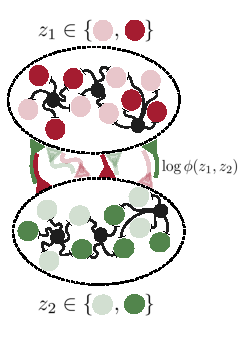
\includegraphics[width=\textwidth]{figures/ch7/example_population2.pdf}
    \label{fig:representation_population}
  \end{subfigure}
  \begin{subfigure}[b]{1.9in}
    \centering
    \caption{}
    \vspace{-.3in}
    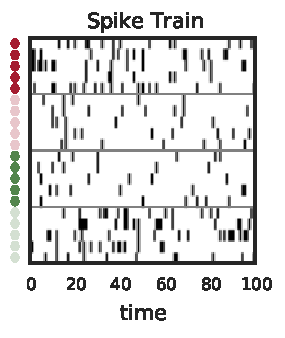
\includegraphics[width=\textwidth]{figures/ch7/example_spiketrain}
    \label{fig:representation_spiketrain}
  \end{subfigure}
  \begin{subfigure}[b]{1.8in}
    \centering
    \caption{}
    \vspace{-.3in}
    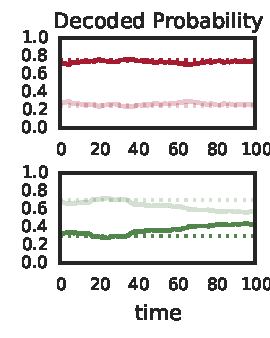
\includegraphics[width=\textwidth]{figures/ch7/example_prs}
    \label{fig:representation_prs}
  \end{subfigure}
  \vspace{-.25in}
  \caption[Example of a population of neurons encoding a probability
    distribution] {Example of a population of neurons encoding marginal
    probability distributions for two binary random variables,~$z_1$
    and~$z_2$. Each variable is represented by a population of neurons,
    which is further divided into subpopulations for each value the variable
    can take on. In~\textbf{(a)},~$z_1$ is represented by red neurons, with
    dark red neurons representing~${z_1=1}$ and light red representing~${z_1=0}$.
    Interneurons (black) provide normalization in the form of local inhibition.
    Excitatory connections between populations implement probabilistic inference.
    \textbf{(b)} The population spike train encodes the marginal distributions.
    For example,~${\Pr(z_1=1)}$ is proportional to the spike count of the subpopulation
    of dark red neurons.
    \textbf{(c)} These probabilities are decoded by integrating
    spike counts for each subpopulation over time and normalizing across
    subpopulations for each variable. Dotted lines: true probability. 
  }
 \label{fig:representation}
\end{figure}


\sloppy
Perhaps the simplest representation of probability is a \emph{direct}
representation in which neural firing rates reflect instantaneous
probabilities. Assume a population of neurons is responsible for
representating the distribution over values that a set of random
variables may take on. We denote this set of variables 
by,~${\bz = \{z_1, \ldots, z_J\}}$.  For
simplicity, assume for now that these variables can only assume a
discrete set of values,~${\{1, \ldots, K\}}$.  \todo{example} Our
neural population is thus tasked with representing probabilty
vectors,~$\bpi^{(j)}$, for each 
variable. The entries of these vectors are,~${\pi^{(j)}_k = \Pr(z_j=k)}$.
\TODO{Later, we will discuss how this representation could be extended
  to allow continuous random variables.}

In a direct representation, each variable-value pair,~$(z_j,k)$, is associated with a population of neurons. The firing
rate of these neurons reflect the instantaneous probability of the
variable taking on that particular value.  Suppose that each
pair, is represented by~$R$ neurons. Moreover, suppose
these representations are \emph{non-overlapping} such that each neuron
can be represented with at most one variable-value pair.
Let~${j_n \in \{1, \ldots, H\}}$
denote the index of the specific variable.
Then, let~$k_n \in \{1, \ldots K\}$ denote the particular value that neuron~$n$ represents.
%A representation size of~$R$ implies that~$\sum_{n=1}^N \bbI[j_n=h] \, \bbI[k_n=k] = R$.

We assume these neurons are stochastic, each endowed
with an instantaneous firing rate,~$\lambda_{t,n}$, which gives rise to an
instantaneous spike count,~$s_{t,n}$ according to a Poisson distribution,
\begin{align}
s_{t,n} &\sim \distPoisson(\lambda_{t,n}).
\end{align}

In a direct representation, the relative spike counts encode
instantaneous probability distributions for each variable. 
If neurons representing a particular value fire twice as many 
spikes as neurons representing a competing value, then the first 
value is twice as likely. We introduce the notion of an 
\emph{integration time},~$T_I$, over which spikes are counted 
to estimate the probability distribution. Then, the empirical 
distribution,~$\widehat{\bpi}_t^{(j)}$, is defined by,
\begin{align}
  \widehat{\pi}_{t,k}^{(j)} &=
  \frac{\sum_{\Delta = 1}^{T_I} \sum_{n=1}^N \bbI[j_n=j] \, \bbI[k_n=k] \, s_{t-\Delta,n}}
       {\sum_{\Delta = 1}^{T_I} \sum_{n=1}^N \bbI[j_n=j] \, s_{t-\Delta,n}}.
\end{align}
The numerator counts spikes from neurons representing the particular value,~$z_j=k$;
the denominator counts all spikes from neurons representing~$z_j$.

Even without any knowledge of the dynamics that gave rise
to these instantaneous firing rates and to the
encoded probability distribution, we can evaluate the complexity
of this representation. How many neurons, time steps, or spikes
are required to guarantee that the encoded distribution is within
some tolerable error of the underlying ground truth? The answer
to this question can provide some important constraints on the
viability of this approach and aid in our search for neural
susbtrates of inference. 

\section{Complexity of Direct Representations}
The stochasticity of the spike counts means that any instant in time,
the probability distribution that is represented by the population
will be a random variable.  First, we will show that this
representation is unbiased. That is, if the firing rates,~$\lambda_{t,
  n}$, are proportional to the probability,~$\pi_{k_n}^{(j_n)}$, then
the represented probability,~$\widehat{\bpi}_{t}^{(j)}$, will have the
correct expectation.  Since we will be focusing on the representation
of a single random variable $z_j$, we drop the superscript~$(j)$ for
the remainder of this section.

\begin{lemma}
\label{lem:consistency}
If the firing rates are proportional to a given probability
distribution over the integration time window then the probability
distribution represented by the population will have expectation equal
to the given probability distribution.  That is,
if~$\lambda_{t, n}=\lambdamax \pi_{k_n}$,
then~$\bbE[\widehat{\pi}_{t,k}] = \pi_{k}$.
\end{lemma}

\begin{proof}
  Let,
  \begin{align}
    S_{t,k} &= \sum_{\Delta = 1}^{T_I} \sum_{n=1}^N \bbI[j_n=j] \, \bbI[k_n=k] \, s_{t-\Delta,n},
  \end{align}
  and
  \begin{align}
    S_{t} &= \sum_{\Delta = 1}^{T_I} \sum_{n=1}^N \bbI[j_n=j] \,  s_{t,n} = \sum_{k=1}^K S_{t,k}.
  \end{align}
  Iterating expectations, we have,
  \begin{align}
    \bbE[\widehat{\pi}_{t,k}] &=
    \bbE \left[ \frac{S_{t, k}}{S_{t}} \right]
    = \bbE \left[
      \bbE \left[
        \frac{S_{t,k}}{S_t} \, \bigg|\, S_{t}  
      \right] \right].
  \end{align}
  Since~$s_{t, n}$ are independent Poisson random variables, their partial
  sums are as well.  Specifically,
  \begin{align}
    S_{t,k} &\sim \distPoisson \left( \sum_{\Delta = 1}^{T_I} \sum_{n} \bbI[j_n=j] \bbI[k_n=k] \lambda_{t,n} \right) \\
    &= \distPoisson \left(\lambdamax T_I \sum_n \bbI[j_n=j] \bbI[k_n=k] \, \pi_{k} \right) \\
    \label{eq:S_t_rate}
    &= \distPoisson(\lambdamax \, T_I \, R \, \pi_{k}),
  \end{align}
  which implies,
  \begin{align}
    S_{t} = \sum_{k} S_{t,k} &\sim \distPoisson(\lambdamax \, T_I \, R).
  \end{align}
  Moreover, their conditional distribution is binomial.
  \begin{align}
    S_{t,k} \given S_t &\sim
    \distBinomial \left( S_t, \frac{\lambdamax \, T_I \, R \, \pi_{k}}{\lambdamax \, T_I \, R} \right)
    =\distBinomial(S_t, \pi_{k}),
  \end{align}
  which has expectation~$\pi_{k} \, S_t$.
  Plugging this into the iterated expectation above, 
  \begin{align}
    \bbE[\widehat{\pi}_{t,k}]
    &= \bbE \left[
      \bbE \left[
        \frac{S_{t,k}}{S_t} \, \bigg|\, S_t  \right] \right] \\
    &= \bbE \left[ 
      \frac{\pi_{k} S_t}{S_t} \right]\\
    &= \pi_{k}.
  \end{align}
  Thus, this procedure is unbiased.
\end{proof}

While this stochastic representation may have the correct expectation, we
would like to characterize the probability that it is ``close'' to its
mean. As we hypothesized above, the difference between the true
probability and that represented by the population should shrink as
the number of spikes grows. We quantify this with the following
theorem, which provides an upper bound on the number of spikes
required to guarantee that the represented probability differs from
the true probability by more than~$\epsilon$. We measure this
difference with the total variation distance between the
distributions,
\begin{align}
  \dtv(\widehat{\bpi}_t, \bpi) &= 
  \max_{\ell} |\widehat{\pi}_{t,k} - \pi_{k}|.
\end{align}

\begin{theorem}
\label{thm:fixed_count}
Given a fixed probability vector~$\bpi$, firing
rates~$\lambda_{t,n} = \lambdamax \pi_{k_n}$ over the integration
time window, a fixed error level~$\epsilon < 1$, and a desired
confidence~$\delta < 1$, there exists a minimum number of spikes~$S^*$
such that if~$S_t \geq S^*$, the conditional probability of error is
bounded
by~$\Pr(\dtv(\widehat{\bpi}_t, \bpi) > \epsilon \given S_t) <
\delta$.  Furthermore, this minimum number of spikes is at most,
\begin{align}
S^* &\leq \frac{1}{2\epsilon^2} \ln \frac{2K}{\delta},  
\end{align}
\end{theorem}

\begin{proof}
First, consider the probability that a particular entry differs from its mean by more than~$\epsilon$.
\begin{align}
  &\Pr(|\widehat{\pi}_k - \pi_k |  > \epsilon \given S_t) \\
  &\qquad= \Pr(\widehat{\pi}_k - \pi_k  > \epsilon \given S_t) + 
  \Pr(\widehat{\pi}_k - \pi_k  < -\epsilon \given S_t) \\
  &\qquad= \Pr \left(S_{t, k} > S_t \pi_{ k} \left(1+\frac{\epsilon}{\pi_{ k}} \right) \, \bigg| \, S_t \right) 
  +\Pr \left(S_{t, k} < S_t \pi_{ k} \left(1-\frac{\epsilon}{\pi_{ k}} \right) \, \bigg| \, S_t\right) \\
  &\qquad= \Pr \left(S_{t, k} > \bbE[S_{t,k} \given S_t] \left(1+\frac{\epsilon}{\pi_{ k}} \right) \right) 
   +\Pr \left(S_{t, k} < \bbE[S_{t,k} \given S_t] \left(1-\frac{\epsilon}{\pi_{ k}} \right) \right)
\end{align}
As in Lemma~\ref{lem:consistency}, we have used the fact
that~$S_{t, k} \given S_t \sim \distBinomial(S_t, \pi_{ k})$,
and hence has expectation~$S_t \pi_{ k}$. 
The probability of this binomial random variable exceeding its mean 
by a multiplicative constant is a decreasing function of the 
number of spikes,~$S_t$. This implies that there exists a minimum 
number of trials~$S^*$ such that for~$S_t \geq S^*$, this probability 
of error is bounded above by~$\delta$, hence proving the first part 
of the theorem.

Now suppose~$S_t=S^*$.  We use a Chernoff bound to upper bound the
probability that the binomial random variable,~$S_{t,k}$, deviates
from its mean by more than a multiplicative factor. Leveraging the
fact that~$\pi_{k} \leq 1$, we have,
\begin{align}
  \Pr \left(S_{t,k} > \bbE[S_{t,k} \given S^*] \left(1+\frac{\epsilon}{\pi_{k}} \right) \right) 
  &\leq \exp \left \{-2S^* \epsilon^2 \right \}, \\
  \Pr \left(S_{t,k} < \bbE[S_{t,k} \given S^*] \left(1-\frac{\epsilon}{\pi_{k}} \right) \right) 
  &\leq \exp \left \{-2S^* \epsilon^2 \right \},
\end{align}
which together imply,
\begin{align}
  \Pr(|\widehat{\pi}_{t,k} - \pi_{k} |  > \epsilon \given S^*) 
  &\leq 2 \exp \left \{-2S^* \epsilon^2 \right \}.
\end{align}
We bound the maximum deviation of any entry in~$\widehat{\bpi}$ with a union bound,
\begin{align}
  \Pr(\dtv(\widehat{\bpi}_t, \bpi) > \epsilon \given S^*) 
  & \leq 2K \exp \left\{-2S^* \epsilon^2 \right\}.
\end{align}
Setting this probability equal to~$\delta$ yields the desired bound on~$S^*$,
\begin{align}
  S^* &\leq \frac{1}{2\epsilon^2} \ln \frac{2K}{\delta}.
\end{align}

\end{proof}


This theorem provides an upper bound on the minimum number of spikes necessary to 
guarantee that the total variation distance between the true and estimated 
probability vectors is less than~$\epsilon$ with probability~$1-\delta$. 
Notably, the relevant quantity is the number of spikes~$S_t$, rather than 
the number of neurons. Thus, there is some flexibility in how the probability 
is estimated: a small population of neurons could be measured over many time bins,
or a large population could be measured over a single time bin. Moreover, the 
population gain,~$\lambdamax$, could be varied to adjust the number of spikes 
per time bin. 

In practice, the number of spikes cannot be set directly. It, is a
Poisson random variable whose mean, from Eq.~\ref{eq:S_t_rate},
is~$\bbE[S_t] = \lambdamax T_I R$: the expected number of spikes per neuron times the number of neurons per
outcome. This leads to the following theorem, which specifies a upper bound 
on the gain and number of neurons required to guarantee that the 
total variation distance is less than~$\epsilon$ with probability~$1-\delta$.

\begin{theorem}
  \label{thm:rate_bounds}
  Given a fixed probability vector~$\bpi$, firing
  rates~$\lambda_{t,n} = \lambdamax \pi_{k_n}$, a fixed error
  level~$\epsilon < 1$, and a desired confidence~$\delta < 1$, the
  probability of error is bounded
  by~$\Pr(\dtv(\widehat{\bpi}_t, \bpi) > \epsilon) < \delta$
  if~$\lambdamax T_I R \geq \mu^*$, where~$\mu^*$ is at most,
  \begin{align}
    \mu^* &\leq \frac{1}{1-e^{-2\epsilon^2}} \ln \frac{2K}{\delta}.  
  \end{align}
\end{theorem}

\begin{proof}
  We have, 
  \begin{align}
    \Pr(\dtv(\widehat{\bpi}_t, \bpi) > \epsilon) 
    &= \sum_{m=0}^\infty \Pr(S_t=m) \Pr(\dtv(\widehat{\bpi}_t, \bpi) > \epsilon \given S_t=m) \\
    &\leq \sum_{m=0}^\infty  \Pr(S_t=m) \times 2K \exp \left \{-2m\epsilon^2 \right\} \\
    &= 2K \bbE_{S_t} \left[ \exp \left \{ -2S_t \epsilon^2 \right \} \right] \\
    &= 2K \exp \left \{\mu^* (e^{-2\epsilon^2}-1) \right\},
  \end{align}
  where the last line follows from moment generating function of~${S_t \sim \distPoisson(\mu^*)}$.
  Setting this equal to~$\delta$ and solving for~$\mu^*$ yields the stated bound.
\end{proof}

% This bound states that for a fixed gain factor, the number of neurons
% required to guarantee that the total variation distance between the
% true and estimated distributions is bounded by~$\epsilon$ could grow
% extremely rapidly as~$\epsilon$ goes to zero.

So far we have considered the estimated probability distribution
obtained by ``reading out'' the entire population of neurons. What if
we only observe a fraction of the population, as a neuron in a
downstream population might? Assume each neuron in the population is 
``observed'' with probability~$\rho$. The expected number of observed 
neurons for a given variable-value pair is~$R\rho$, and if we see 
exactly the expected number of neurons for each value, the estimated 
probability distribution will have the correct expectation. However, 
in practice we will incur some bias from seeing a different number of 
neurons for each value. Bounding the error theoretically is challenging 
due to this additional source of randomness, so we instead consider 
the simple case in which we see exactly~$R \rho$ neurons for each value.
Then, following the same logic as above, we have the following 
corollary.

\begin{corollary}
  \label{cor:sparse_bounds}
  Given a fixed probability vector~$\bpi$, firing
  rates~$\lambda_{t,n} = \lambdamax \pi_{k_n}$ over the
  integration time window, a fixed error level~$\epsilon < 1$, and a
  desired confidence~$\delta < 1$, and~$\rho R$ observed neurons for
  each of the~$K$ values, the probability of error is bounded
  by~$\Pr(\dtv(\widehat{\bpi}_t, \bpi) > \epsilon) < \delta$ if
  \begin{align}
    (\lambdamax T_I) (\rho R) \geq \mu^*,
  \end{align} 
  where~$\mu^*$ is at most,
  \begin{align}
    \mu^* &\leq \frac{1}{1-e^{-2\epsilon^2}} \ln \frac{2K}{\delta}.  
  \end{align}
\end{corollary}

\begin{proof}
  This follows directly from Theorem~\ref{thm:rate_bounds} with $\rho R$ substituted for~$R$.
\end{proof}

Corollary~\ref{cor:sparse_bounds} provides theoretical connection
between the fidelity of the representation, measured in terms of the
error~$\epsilon$ and confidence~$\delta$ for a given number of
values~$K$, and parameters of the neural implementation, namely the
maximum firing rate, the integration time, the connection probability,
and the representation size.  The expected spike count is the product
of the effective number of neurons,~$\rho R$, and the expected number
of spikes per neuron,~$\lambdamax T_I$.  Together, these allow us to
deduce a manifold of trade-offs between population size and
integration time that will achieve a desired error level and
confidence. 


% Figure: Theoretical bounds on error and physiological parameters
\begin{figure}[t!]
  \centering
  \begin{subfigure}[b]{2.75in}
   \centering
   \caption{}
   \vspace{-.4in}
   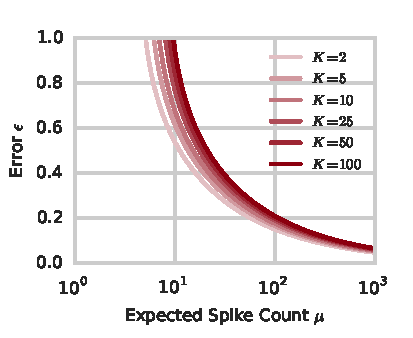
\includegraphics[width=\textwidth]{figures/ch7/error_vs_expected_spike_count}
   \label{fig:error_vs_expected_spike_count}
 \end{subfigure}
 \begin{subfigure}[b]{2.75in}
   \centering
   \caption{}
   \vspace{-.4in}
   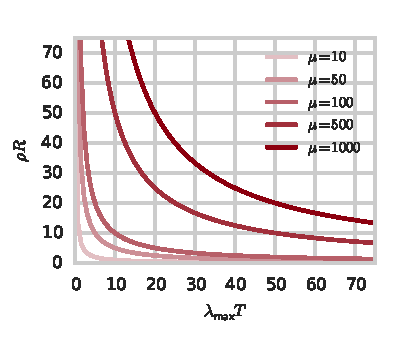
\includegraphics[width=\textwidth]{figures/ch7/mu_for_R_T}
   \label{fig:mu_vs_R_T}
 \end{subfigure}
 \vspace{-.3in}
 \caption[Theoretical bounds on expected spike count and physiological parameters]
 { Theoretical relationship between between total variation distance, expected spike
   count, and physiological parameters. 
   \textbf{(a)} Theoretical 
   upper bound on the 95th percentile of the total variation distance,~$\epsilon$, 
   as a function of the expected spike count,~$\mu = (\rho R) (\lambdamax T_I)$,
   for increasing values of~$K$. 
   \textbf{(b)} The expected spike count is the product of the effective number 
   of neurons,~$\rho R$, and the effective number of spikes per neuron,~$\lambdamax T_I$.
   This shows how time and number of neurons can be balanced to obtain the desired 
   expected spike count.
 }
 \label{fig:theoretical_complexity}
\end{figure}

Figure~\ref{fig:theoretical_complexity} plots these theoretical 
bounds. Fig.~\ref{fig:error_vs_expected_spike_count} shows the theoretical
upper bound on the 95th percentile of the total variation distance as a
function of the expected spike count for a range of distribution sizes,~$K$.
Fig.~\ref{fig:mu_vs_R_T} illustrates the trade-offs between effective 
number of neurons and expected number of spikes per neuron necessary 
to achieve a desired expected spike count.


% Figure: empirical and theoretical total variation distance
\begin{figure}[t!]
  \centering
  \begin{subfigure}[b]{2.75in}
    \centering
    %\caption{}
    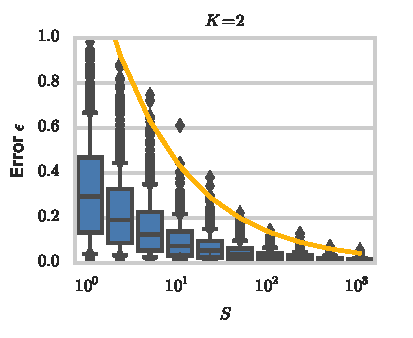
\includegraphics[width=\textwidth]{figures/ch7/error_vs_S_K2}
    \label{fig:error_vs_S_K2}
 \end{subfigure}
 \begin{subfigure}[b]{2.75in}
   \centering
   %\caption{}
   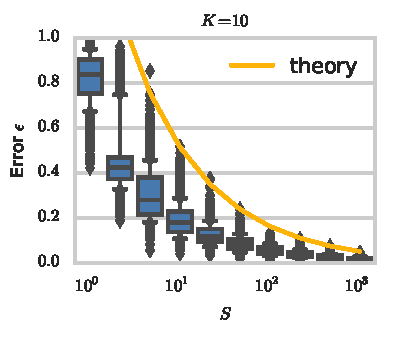
\includegraphics[width=\textwidth]{figures/ch7/error_vs_S_K10}
   \label{fig:error_vs_S_K10}
 \end{subfigure}
 \\
 \vspace{-.25in}
 \begin{subfigure}[b]{2.75in}
   \centering
   %\caption{}
   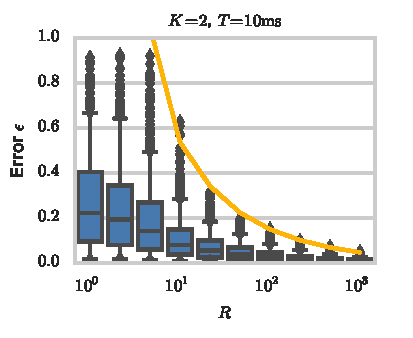
\includegraphics[width=\textwidth]{figures/ch7/error_vs_R_K2}
   \label{fig:error_vs_R_K2}
 \end{subfigure}
 \begin{subfigure}[b]{2.75in}
   \centering
   %\caption{}
   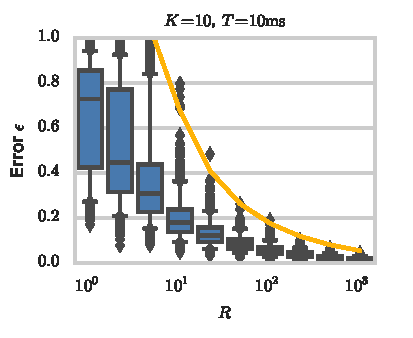
\includegraphics[width=\textwidth]{figures/ch7/error_vs_R_K10}
   \label{fig:error_vs_R_K10}
 \end{subfigure}
 \\
 \vspace{-.25in}
 \begin{subfigure}[b]{2.75in}
   \centering
   %\caption{}
   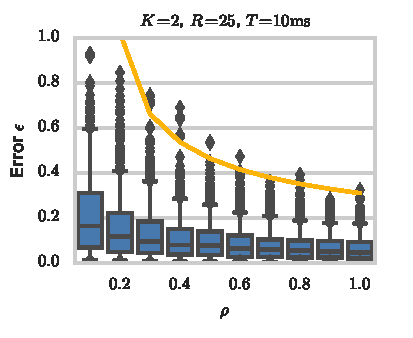
\includegraphics[width=\textwidth]{figures/ch7/error_vs_rho_K2}
   \label{fig:error_vs_rho_K2}
 \end{subfigure}
 \begin{subfigure}[b]{2.75in}
   \centering
   %\caption{}
   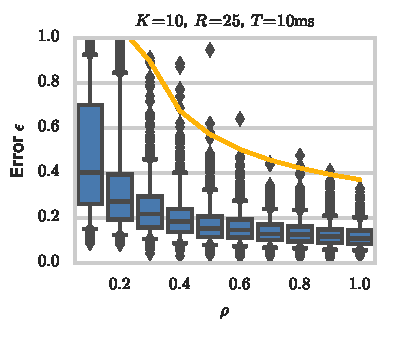
\includegraphics[width=\textwidth]{figures/ch7/error_vs_rho_K10}
   \label{fig:error_vs_rho_K10}
 \end{subfigure}
 \vspace{-.3in}
 \caption[Empirical and Theoretical Total Variation Distance]
 {Empirical and theoretical total variation distance under a variety 
   of parameter regimes. Whiskers show the empirical~5th 
   and~95th percentiles. Yellow line shows the theoretical
   upper bound on the 95th percentile. 
   \textbf{Left} column:~$K=2$. \textbf{Right} column:~$K=10$. 
   \textbf{Top} row: fixed population spike count,~$S$. 
   \textbf{Middle} row: varying the number of neurons per variable.
   \textbf{Bottom} row: varying the connection probability.
   See text for full description.
 }
 \label{fig:complexity}
\end{figure}

Figure~\ref{fig:complexity} shows the results of an empirical 
assessment of this theory under a variety of parameter regimes.
For each regime, we show the results for discrete distributions over
~$K=2$ values (left column) and~$K=10$ values (right column). We 
sample~$1000$ discrete distributions from a Dirichlet 
prior,~${\bpi \sim \distDirichlet(\bone_K)}$, and then we encode each true 
distribution with Poisson spiking neurons and measure the total 
variation distance between the true and encoded distributions. 

In the top row, we consider the case where the total population 
spike count is set explicitly, as in Theorem~\ref{thm:fixed_count}.
In this case, the spikes are attributed to each value according 
to a multinomial distribution. We plot the theoretical bound from
Theorem~\ref{thm:fixed_count} in yellow.

In the middle row we measure the error as a function of the
representation size,~$R$, for~$\rho=1.0$, under the assumption that
spikes are counted in one millisecond bins for~$T_I=10$ milliseconds,
and a maximum firing rate of~$100$Hz (i.e.~$\lambdamax=0.1$). Thus, in
expectation the population will emit~$R$ spikes, allowing the top and
middle rows to be directly compared. That is, in the top row, the
population fires exactly the number of spikes expected in the middle
row.  We see that the stochastic population spike counts does indeed
introduce extra variability in the error, as predicted by
Theorem~\ref{thm:rate_bounds}, though the median error is not
substantially different from that of the fixed-$S$ case.

Finally, the bottom row shows the empirical and predicted error as 
we vary the observation probability,~$\rho$. Here, the representation 
size is fixed to~$R=25$, and the gain and integration time are 
set as in the middle row. While a strict upper bound is difficult 
to derive theoretically, the approximation from 
Corollary~\ref{cor:sparse_bounds} provides a reasonable 
approximation for this parameter regime.

These complexity-theoretic bounds relate the number of spikes to the 
total variation distance between the true and estimated distributions.
From the number of spikes, we can deduce constraints on the representation
size, integration time, and connection probability, for realistic gain levels.
While the theoretical bounds do not exactly match the empirical error 
distributions, they appear to be roughly correct up to a multiplicative 
factor. Thus, if we can estimate some biophysical properties like 
connection probabilities, integration times, and firing rates, 
and we can constrain the error 
tolerances of the algorithms that consume these probability estimates, 
then we can estimate the number of neurons that must represent 
each variable-value pair. This will prove useful in guiding our 
bottom-up search, and serve as an important constraint for assessing 
the viability of a direct representation of probability.


% Inference section
\section{Bayesian Inference with Neural Dynamics}
\label{sec:inference}
Two forces cause the encoded distributions to change over time. As
we interact with the world and receive new inputs, the probabilities
of the visible variables change to reflect the new
observations. Moreover, even for a fixed set of visible variable
assignments, the probabilities of hidden variables will change as we
perform inference. Bayesian inference is the process of computing the
posterior distribution over latent variables given the values of visible
inputs. Many inference algorithms are iterative. Thus, as the
algorithms execute, the instantaneous probability distribution will
vary. Next, we describe how a simple inference algorithm can be
implemented with biologically plausible neural dynamics.

We assume that as an organism receives new inputs from the world, it
updates its posterior distribution over the values of latent
variables. Doing so requires a probabilistic model that relates hidden
and observed variables via a joint probability distribution.  Whereas
in previous chapters we have considered directed graphical models,
here we assume that the probabilistic models implemented in the brain
are best described in terms of a \emph{factor graph},
\begin{align}
  \label{eq:probabilistic_model}
  p(\bz \given \btheta) &=
  \frac{1}{Z(\btheta)}
  \prod_{j \in \mcG} \phi(z_j \given \btheta) \,
  \prod_{i,j \in \mcG} \phi(z_i, z_j \given \btheta) \,
\end{align}
Here, the graph,~$\mcG$, specifies pairs of variables with
probabilistic dependencies.  Each unary factor,~$\phi(\cdot \given
\btheta)$ is a function that maps a variable assignment to a
nonnegative real number, and each pairwise factor,~$\phi(\cdot, \cdot
\given \btheta)$, is a function that maps a pair of assignments,
say~${(z_i=k, z_j=k')}$ to a nonnegative real number. The
normalizing constant,~$Z(\btheta)$, ensures that the joint probability
distribution sums to one.

The probabilistic model in Eq.~\ref{eq:probabilistic_model} reflects
a specific assumption about the types of dependency structures
neural populations can represent.

\begin{assumption}
  Neural populations only perform inference in probabilistic models
  that factor into the product of unary and pairwise dependencies. 
\end{assumption}

A typical model need not factor into pairwise terms. It may instead
have factors that relate three or more latent variables. As we will
see, unary and pairwise factors map naturally onto neural biases
and synaptic weights. In our proposed neural implementation, higher
order factors would require the interaction of three or more neurons.
While this may be realized with dendritic computation or interneurons,
these more sophisticated implementations are beyond the scope of this
chapter. 

In general, the posterior distribution of a subset of hidden
variables~$\bz_H \subseteq \bz$ 
given the observed variables~$\bz_O = \bz \setminus \bz_H$ is,
\begin{align}
  p(\bz_H \given \bz_O, \btheta) &=
  \frac{p(\bz_H, \bz_O \given \btheta)}
       {\sum_{\bz_H} p(\bz_H, \bz_O \given \btheta)},
\end{align}
cannot be efficiently computed since it requires a sum over all
possible hidden variable assignments.
However, as we have seen in previous chapters, there are many methods of
approximating posterior distributions. Mean field variational
inference  maps particularly nicely onto the natural constraints
of neural dynamics. 
In mean field variational inference, the exact (but intractable)
posterior distribution is approximated with a factorized
distribution,
\begin{align}
  p(\bz_H \given \bz_O, \btheta) &\approx q(\bz_H) \equiv \prod_{z_j \in \bz_H} q(z_j).
\end{align}
The terms in this product are called \emph{variational factors}.  We
solve for the variational factors that minimize KL-divergence between
the true and approximate posterior,~$\KL(q(\bz_H) \,||\, p(\bz_H
\given \bz_O, \btheta))$. In minimizing the KL-divergence, we
simultaneously maximize a lower bound on the marginal log
likelihood,~$\log p(\bz_O \given \btheta)$.

The simplest method of minimizing this objective is via coordinate
descent, iteratively updating the probability of one hidden variable
given the probabilities of the rest. Since our variational
distribution is factorized, the variational factor for variable~$j$
must satisfy the mean field consistency equation:
\begin{align}
  \label{eq:mf_consistency}
  \log q(z_j) &\simeq \bbE_{q(\bz_{\neg j})}
  \left[ \log p(\bz_H, \bz_O \given \btheta) \right],
\end{align}
where~$\simeq$ denotes equality up to an additive constant and the
expectations are taken with respect to the variational
distribution over other hidden variables,
\begin{align}
  q(\bz_{\neg j}) &= \prod_{i \neq j} q(z_{i}).
\end{align}
The additive constant
ensures normalization of the probabilities, and will be discussed
subsequently.  

For discrete random variables, the variational factors are simply
vectors specifying the posterior probability of each variable,~$z_j$.
Under the direct representation described above, these instantaneous
values of these factors are encoded in the relative spike counts of
populations of neurons,
\begin{align}
  q_t(z_j=k) &= \widehat{\pi}_{t,k}^{(j)} 
\end{align}
To perform inference, the neuronal dynamics must be such that at each
time step, the relative spike counts satisfy~Eq.~\ref{eq:mf_consistency}. 
%For discrete random variables, this implies that the rate of a neuron~$n$
%that represents the variable-value pair~(${j_n=j,\,k_n=k}$) should obey,
Explicitly writing the additive constant,~$-\log \nu_t^{(j)}$, we have,
\begin{align}
  \nonumber
  \log \widehat{\pi}_{t,k}^{(j)} 
  &= -\log \nu_t^{(j)} + \log \phi(z_j=k \given \btheta) \\
  &\hspace{4em} + \bbE_{q_{t-1}(\bz_{\neg j})} \bigg[
  \sum_{i \in \neigh(j)} \log \phi(z_{i}, z_j=k \given \btheta) \bigg] \\
  % In terms of firing rates
  & \nonumber = 
     - \log \nu_t^{(j)} + \log \phi(z_j=k \given \btheta) \\
  & \label{eq:variational_rate}
  \hspace{4em} + \sum_{i \in \neigh(j)} \sum_{k'=1}^K
  \bigg[\log \phi(z_{i}=k', z_j=k \given \btheta) \,\cdot  \widehat{\pi}_{t-1,k'}^{(i)} \bigg] \\
  &= -\log \nu_t^{(j)} + \psi_{t,k}^{(j)}.
\end{align}
where we have combined the terms from the unary and pairwise factors
into the activation,~$\psi_{t,k}^{(j)}$.

Since~$\widehat{\bpi}_{t}^{(j)}$ is a probability distribution, we
know it must sum to one. Thus the additive constant must be set to
ensure this normalization.  Thus,
\begin{align}
  \widehat{\pi}_{t,k}^{(j)} &=
  \exp \left \{\psi_{t,k}^{(j)} -\log \nu_{t}^{(j)} \right \},
  & & &
  \nu_t^{(j)} &= \sum_{k'} \exp \left \{\psi_{t,k'}^{(j)} \right \}.
\end{align}

%Note that the pairwise factor functions are not necessarily symmetric.
%In fact, the two variables may have support for different ranges of
%values, so symmetry often does not make sense.  We have written this
%such that~$z_j$ is always the second argument, but its order will
%depend on its role in each factor.

Now that we have derived theoretically exact mean field updates, we
must show how they can be approximated with plausible neural dynamics.
We assume that inference occurs on a characteristic time scale of~$T_I$
time steps. This reflects the window of time over which neurons estimate
probability distributions.
From Lemma~\ref{lem:consistency}, we know that if the firing rates of
neurons the variable-value pair~${(z_j,k)}$ are proportional
to~$\widehat{\pi}_{t,k}^{(j)}$, then in expectation, the empirical
distribution represented by the spike counts will be equal to the
desired distribution. Thus, we aim to set,
\begin{align}
  \lambda_{t,n} &= \lambdamax \, \widehat{\pi}_{t,k_n}^{(j_n)}
  = \lambdamax \exp \left \{\psi_{t,k_n}^{(j_n)} -\log \nu_{t}^{(j_n)} \right \},
\end{align}
for maximum firing rate,~$\lambdamax$. While this rate function is
nearly a linear-nonlinear cascade, as we studied in previous
chapters, there is one major impediment to realizing this
calculation in biological neurons. Specifically, to compute
the activation, a neuron must have access to the \emph{normalized}
probabilities of other hidden and visible variables. In practice,
a neuron only observes the spike counts of the neurons it receives 
input from. However, these can be used to estimate the desired probabilities.
This motivates our next assumptions,

\begin{assumption}
  Neurons are sparsely connected to one another. For each directed
  pair of neurons, $(n,m)$, the variable~$a_{n \from m} \in \{0,1\}$
  indicates whether or not there exists a synaptic connection from
  neuron~$m$ to neuron~$n$. These connections are modeled as
  independent and identically distributed Bernoulli random variables,
  \begin{align}
    a_{n \from m} &\sim \distBernoulli(\rho).
  \end{align}
  We combine these variables into a binary adjacency 
  matrix,~$\bA \in \{0,1\}^{N \times N}$.
\end{assumption}

\begin{assumption}
  All neurons in the population share the same gain,~$\lambdamax$. 
  Thus, neuron~$n$'s estimate of~$\bpi^{(j)}$ is 
  informed by~$(\lambdamax T_I)(\rho R)$ spikes, in expectation:
  \begin{align}
    \bbE_{\bA,\bs} \bigg[ \sum_{\Delta = 1}^{T_I} & \sum_{m=1}^N \bbI[j_m=j] \, a_{n \from m} \cdot s_{t-\Delta,m} \bigg] \\
    &= \bbE_{\bA,\bs} \left[ \sum_{\Delta = 1}^{T_I} \sum_{m=1}^N \sum_{k=1}^K \bbI[j_m=j] \, \bbI[k_m=k] \, a_{n \from m} \cdot s_{t,m} \right] \\
    &= \lambdamax T_I \rho \sum_{m=1}^N \sum_{k=1}^K \bbI[j_m=j] \, \bbI[k_m=k] \, \widehat{\pi}_{t,k}^{(j)} \\
    &= (\lambdamax T_I) (\rho R).
  \end{align}

  Moreover, the instantaneous probability is well-approximated by,
  \begin{align}
      \widehat{\pi}_{t,k}^{(j)} &=
  \frac{\sum_{\Delta=1}^{T_I} \sum_{m=1}^N \bbI[j_m=j] \, \bbI[k_m=k] \, a_{n \from m} \cdot s_{t-\Delta, m}}
       {\sum_{\Delta=1}^{T_I} \sum_{m=1}^N \bbI[j_m=j] \, a_{n \from m} \cdot s_{t-\Delta, m}} \\
       &\approx (\lambdamax T_I \rho R)^{-1} \sum_{\Delta=1}^{T_I} \sum_{m=1}^N \bbI[j_m=j] \, \bbI[k_m=k] \, a_{n \from m} s_{t-\Delta, m}.
  \end{align}
  In other words, the total spike count is concentrated around its mean.
\end{assumption}

Under the assumption of shared gain, the
desired dynamics in~Eq.~\ref{eq:variational_rate}
simplify to,
\begin{align}
  \label{eq:mf_log_probs}
  \lambda_{t,n} &= \lambdamax
  \exp \left \{b_n + (\lambdamax T_I \rho R)^{-1} \sum_{\Delta=1}^{T_I} \sum_{m=1}^N a_{n \from m} \cdot w_{n \from m} \cdot s_{t-\Delta,m}
  - \log \nu_t^{(j_n)} \right \}
\end{align}
where
\begin{align}
  b_n &= \log \phi(z_{j_n} = k_n \given \btheta),
\end{align}
and
\begin{align}
  w_{n \from m} &=
  \begin{cases}
    \log \phi(z_{j_n}=k_n, z_{j_m}=k_m \given \btheta) & \text{if }j_m
    \in \neigh(j_n) \\
    0 & \text{o.w.}
  \end{cases}
\end{align}

The last step is to compute the normalizing input,~$\nu_t^{(j)}$.
This requires summing the instantaneous rates of all neurons representing the
random variable,~$z_j$. While this is clearly implausible, we may derive
a gain controller from an alternative perspective. Normalizing the
probability distribution ensures that the expected spike count at
any time step for
neurons representing~$z_j$ is equal to~$\lambdamax R$. If the distribution
is not properly normalized, the expected spike count will deviate.
Thus, a reasonable gain controller can estimate the population
can estimate the population rate,
\begin{align}
\widehat{\lambda}_{t}^{(j)} &= \sum_{\Delta = 1}^{T_G} \sum_{n=1}^N \bbI[j_n=j] s_{t-\Delta, n},
\end{align}
and set the control input to,
\begin{align}
  \nu_{t}^{(j)} &= \frac{\widehat{\lambda}_{t}^{(j)}}{\lambdamax T_G R}.
\end{align}
The time scale of the gain controller is typically set to be
less than the time scale of inference, that is~$T_G < T_I$.


This theory provides a normative interpretation of synaptic weights.
Here, synaptic weights reflect the conditional log probabilities
for the variable-value pairs represented by the pre- and post-synaptic
neurons.

\section{Example of a Simple Mixture Model}
\label{sec:mixture_example}

% Figure: Example of neural inference in a simple mixture model
\begin{figure}[t!]
  \centering
  \begin{subfigure}[b]{5.5in}
   \centering
   \caption{}
   \vspace{-.3in}
   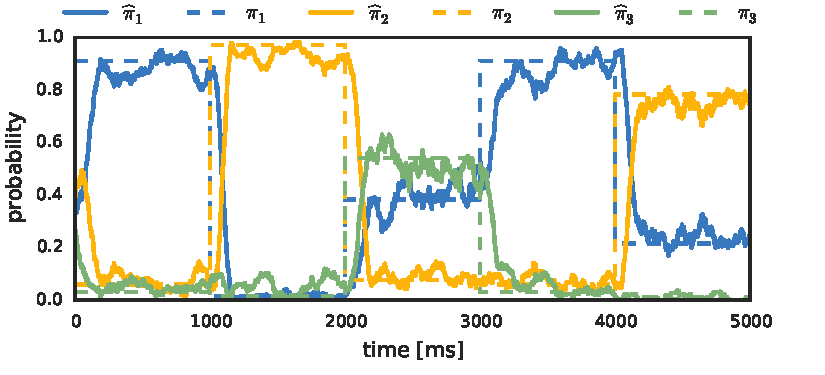
\includegraphics[width=\textwidth]{figures/ch7/neural_mixture_probs}
   \label{fig:mixture_probs}
 \end{subfigure} \\
 \begin{subfigure}[b]{5.5in}
   \centering
   \caption{}
   \vspace{-.4in}
   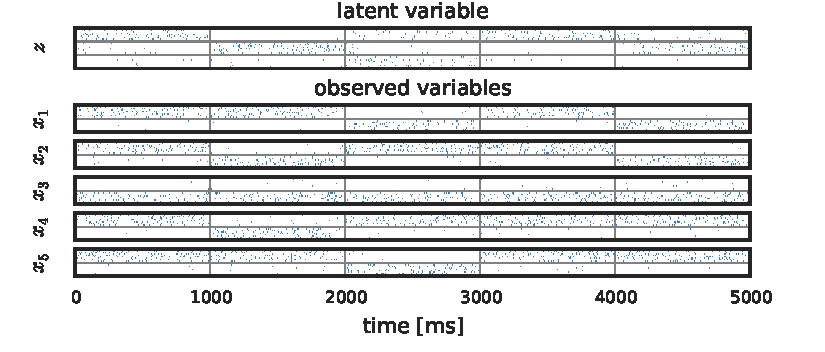
\includegraphics[width=\textwidth]{figures/ch7/neural_mixture_spiketrains}
   \label{fig:mixture_spiketrains}
 \end{subfigure}
 \vspace{-.3in}
 \caption[Demo of neural inference in a simple mixture model]
         {Example of neural inference  a simple mixture model with one
           latent variable,~$z \in \{1, 2, 3\}$, indicating which of the
           three mixture components gave rise to the data. The observations
           consist of 5 conditionally independent binary
           variables,~$x_1, \ldots, x_5$, whose values change every second. 
           %Each variable-value pair is represented by~$R=10$ neurons.
           \textbf{(a)} The empirical probabilities (solid lines) decoded
           from the spike train, and the true posterior (dashed line).
           Stochasticity arises from noisy inputs and Poisson spike counts.
           \textbf{(b)} The underlying spike trains of the neurons representing
           ~$z$ and~$x_i$. Horizontal gray lines distinguish subpopulations of~$R=10$ neurons for
           each value; vertical lines denote times of stimulus change.
 }
 \label{fig:mixture}
\end{figure}


First, we consider a simple mixture model with a single
latent variable denoting the mixture component,~$z \in \{1, \ldots, K\}$,
and a set of conditionally independent observations,~$\{x_j\}_{j=1}^J$.
In this example, we let the observations be Bernoulli
random variables. The model is parameterized by a marginal
class probability vector,~$\balpha$, which we assume is uniform,
and class-conditional probabilities for each observation,
${\rho_{j,k} = \Pr(x_j=1 \given z=k)}$. Together, these
specify the probabilistic model,
\begin{align}
  \balpha &= \tfrac{1}{K} \bone, & & &
    z &\sim \distCategorical(\balpha), \\
  \rho_{j,k} &\sim \distBeta(\tfrac{1}{2},\tfrac{1}{2}),  & & &
  x_j &\sim \distBernoulli(\rho_{j,z}).  
\end{align}
This can be easily transformed into a factor graph with,
\begin{align}
  \phi(z=k) &= \alpha_k, \\
  \phi(x_j=1 \given z=k) &= \rho_{j,k}, \\
  \phi(x_j=0 \given z=k) &= 1-\rho_{j,k}.
\end{align}

We simulate inference in this model with a population of neurons.
Each variable-value pair is represented by~$R=10$ neurons, and each
pair of neurons is connected with probability~$\rho=0.5$. The maximum
firing rate is set to~$\lambdamax=100\text{Hz}$, and the integration
time window is set to~$T_I=100\text{ms}$. Hence, the expected spike
count used to estimate probabilities is~$(\rho R)(\lambdamax T_I)
= 50$ spikes. The neurons representing the observed variable assignment
~$x_j=k$ are externally driven at a rate of~$0.95 \lambdamax$ if~$x_j=k$,
and a rate of~$0.05 \lambdamax$ if~$x_j=\neg k$. We assume that the
synaptic weights have already been learned and reflect the exact
log of the pairwise factors. 

Figure~\ref{fig:mixture} illustrates inference dynamics for a
changing stimulus. Every second, the observed variables are driven with
a new pattern, which leads to a new posterior distribution over the
latent variable. With each change in input, the neurons representing the
latent variable adjust their firing rates to reflect this new probability.
Fig.~\ref{fig:mixture_probs} shows the decoded probabilities over time
(solid lines) along with the true posterior (dashed lines). Despite many
sources of stochasticity, the decoded probabilities do converge to
the correct posterior values. The $100$ms integration time is reflected in
the delayed convergence upon each change in stimulus.
Fig.~\ref{fig:mixture_spiketrains} shows the spike trains from which these
probabilities were decoded. The neurons are ordered according to
the value they encode and the subpopulations of~$R$ neurons are
separated by horizontal light gray lines. Vertical lines indicate changes
in input. Overall, the neurons fire at between $30$ and $40$Hz, with a
dynamic range of about $0$ to $100$Hz, as expected.



\section{Reverse Engineering the Probabilistic Model from Spike Trains}

Given this ``top-down'' theory of neural computation, can we reverse
engineer the probabilistic model from neural recordings? To do so, we
need to infer the subpopulations of neurons that encode each
variable-value pair, as well as the characteristic weights that
connect each subpopulation.  We show that this is possible using the
generalized linear models and structured network priors described in
Chapter 4.


Recall the theoretical dynamics proposed in Section~\ref{sec:inference},
 reproduced here in slightly simplified form,
\begin{align}
  \lambda_{t,n} &= \lambdamax
  \exp \left \{b_n + \gamma \sum_{\Delta=1}^{T_I} \sum_{m=1}^N a_{n \from m} \cdot w_{n \from m} \cdot s_{t-\Delta,m}
  - \log \nu_t^{(j_n)} \right \}.
\end{align}
The instantaneous firing rate take the form of a generalized linear model.
Each neuron has a baseline rate that is a function of~$b_n$ and~$\lambdamax$.
Moreover, the rate is influenced by recent spiking activity through
the network,~$\bA \odot \bW$, and through the local normalization,~$\nu$. 

According to our theory of neural inference, the sparsity pattern of
the network should follow an independent Bernoulli model. That is,
each edge is present with the same probability,~${a_{n \from m} \sim
  \distBernoulli(\rho)}$.  Moreover, the weights of network should
encode the pairwise log probabilities,~${\log \phi(z_i=k, z_j=k')}$,
and the weights from the~$R$ neurons representing~${z_i=k}$ to the~$R$
neurons representing~${z_j=k'}$ should all be approximately
equal. This corresponds to stochastic block structure in the weight
matrix. Thus, to reverse engineer the probabilistic model from the
observed spike train, we fit a generalized linear model with a
spike-and-slab network prior that has an independent Bernoulli model
for the adjacency matrix, and a stochastic block model (SBM) for the
weight matrix. The SBM has latent variables for each neuron that
indicate the cluster assignment, and parameters that specify the
average weight between each pair of clusters:
\begin{align}
  c_n & \sim \distCategorical(\alpha \bone), \\
  \mu_{c \from c'} &\sim \distGaussian(0, \sigma_0^2), \\
  w_{n \from m} &\sim \distGaussian(\mu_{c_n \from c_m}, \sigma^2).
\end{align}
By performing Bayesian inference in this model, we recover a posterior
distribution over biases,~$\{b_n\}_{n=1}^N$; weighted adjacency
matrices,~$\bA$ and~$\bW$; latent variables,~$\{c_n\}_{n=1}^N$; and
parameters,~$\{\mu_{c \from c'}\}_{c,c'=1}^C$.

The normalization presents a minor complication. According to the
theory, this is most likely computed by local inhibitory neurons
that estimate the population rate of neurons representing~$z_j$
and deliver a common, normalizing input to stabilize the rate
at the desired level. This can be roughly approximated with
direct, excitatory connections between neurons representing the same
variable-value pair, and inhibitory connections between neurons
representing competing values of the same variable. In other words,
if we focus solely on the activity of neurons representing the variable-value
pairs, we should expect additional \emph{functional} connections
that encode the mutually exclusive nature of the distinct values
of a given variable.

% Figure: Example of neural inference in a simple mixture model
\begin{figure}[t!]
  \centering
  \begin{subfigure}[b]{2.75in}
   \centering
   \caption{}
   \vspace{-.3in}
   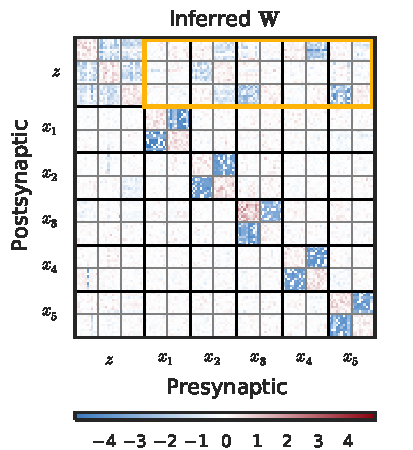
\includegraphics[width=\textwidth]{figures/ch7/mixture_network}
   \label{fig:mixture_network}
  \end{subfigure}
  ~
  \begin{subfigure}[b]{2.75in}
   \centering
   \caption{}
   \vspace{-.3in}
   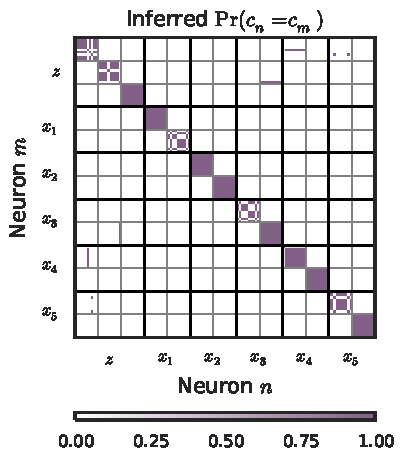
\includegraphics[width=\textwidth]{figures/ch7/mixture_cocluster_probability}
   \label{fig:mixture_cocluster}
 \end{subfigure} \\
 \begin{subfigure}[b]{5.5in}
   \centering
   \caption{}
   \vspace{-.4in}
   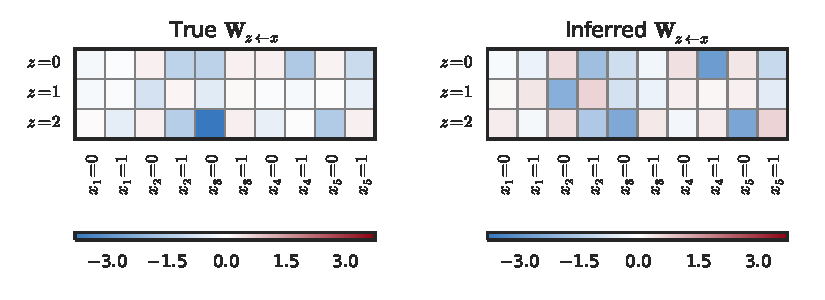
\includegraphics[width=\textwidth]{figures/ch7/mixture_prob_weights}
   \label{fig:mixture_prob_weights}
 \end{subfigure}
 \vspace{-.3in}
 \caption[Reverse engineering probabilistic models from neural spike
   trains] {The probabilistic model can be reverse engineered from the
   neural spike train.
   \textbf{(a)} Inferred weighted adjacency matrix for the population
   of 130 neurons. Thin lines dilineate boundaries between subpopulations
   for each value of~$z$ and~$x_j$; bold lines separate populations for
   each variable. 
   \textbf{(b)} Inferred probability that each pair of neurons belongs to
   the same cluster under a stochastic block model.
   The block diagonal structure shows that the
   variable-value subpopulations are clearly recovered.
   \textbf{(c)} True and inferred weights
   from~$x_j$ to~$z$ (yellow square in~\textbf{(a)}). Inferred weights
   are the mean weights under the stochastic block model. They accurately
   recover the true weights.
 }
 \label{fig:mixture_recovery}
\end{figure}

We demonstrate this approach by 
fitting the hierarchical model to a neural spike train simulated
from the population described in
Section~\ref{sec:mixture_example}. The population performs inference
in a simple mixture model with three latent mixture components,
and five binary observations. An observation consists of an assignment
of the five observations, indicated
by the variables~$\{x_j\}_{j=1}^5$, and given an observation, the dynamics
perform posterior inference of~$z$, the latent variable indicating the
underlying mixture component. The population consists of 130 neurons, 10 for
each variable-value pair.



Figure~\ref{fig:mixture_recovery} shows the inferred parameters of the
hierarchical model. The posterior mean of the weighted adjacency
matrix is shown in Figure~\ref{fig:mixture_network}, with neurons sorted
by variable and then by value. The block diagonal strucutre shows
the normalizing connections betewen neurons representing the same variable,
and the region highlighted in yellow shows the inferred connections from
neurons representing~$x_j$ to neurons reprsenting~$z$. These encode
the pairwise log probabilities of the mixture model.

Figure~\ref{fig:mixture_cocluster} shows the inferred posterior probability
of two neurons belonging to the same cluster. While the true model has
13 clusters, we allowed our model to use as many as 20 clusters.
If the variable-value subpopulations
were recovered perflectly, this matrix would be block diagonal. We
see that it is nearly so; only a handful of neurons are misclassified
and some blocks are split in two.

Finally, Figure~\ref{fig:mixture_prob_weights} shows the true and inferred
mean weights under the stochastic block model. First, we found the permutation
of inferred cluster labels that best matched the true cluster labels. Then we found the
linear transformation that best matched the true and inferred weights.
The result shows that the true pattern of weights from~$x_j$ to~$z$ are
recovered with high fidelity.

While this procedure for reverse engineering probabilistic models
from observed spike trains is not foolproof, this simple example
illustrates that much can be learned by combining top-down theories
with bottom-up analysis. To further improve this inference procedure,
we should include two sets of latent cluster assignments in our
hierarchical model: one set of variables that specifies the
variable that a cluster of neurons represents (i.e.~$j_n$ in our
theory), and another that indicates the value (i.e.~$k_n$).
Incorporating the knowledge that different values of the same variable
are mututally exclusive, we can build a strong prior distribution
over weights given these two variables. 

What else can be learned from the results of this approach? In
practice, we only observe a fraction of the neurons in a particular
region If our recording method samples~$N$ neurons out
of~$N_{\mathsf{total}}$, then given an inferred block
size,~$\widehat{R}$, we can estimate the true representation size to
be roughly,~$R\approx \widehat{R} N_{\mathsf{total}} / N$. If variable-value
subpopulations are truly disjoint, this provides an estimate of the
number of subpopulations the region could encode. Combined with the
complexity theoretic bounds developed in Section~\ref{sec:complexity},
these top-down and bottom-up approaches provide two tacks  by which we may 
converge on a theory of probabilistic inference in neural circuits.

\section{Discussion}

\subsection{More ideas}

\subsubsection{Localization with Hippocampal Place Cells}

Model:
\begin{itemize}
\item Latent locations,~$z_i \in \{1, \ldots, K\}$ for time indices~$-D, \ldots, 0$.
\item Sensory cues,~$x_{i,j} \in \{0,1\}$ for~$j \in \{1, \ldots, J\}$.
\item Transition probability~$\phi(z_{i-1}, z_i)$. How could these weights be shared?
\item Observation probability~$\phi(z_{i}, x_{i,j})$. And how could these be shared?
\end{itemize}

\subsubsection{Olfactory Scene Parsing}


Model:
\begin{itemize}
\item Presence or absence of odorant~$n$ in scene~$d$:~$w_{d,n} \in \{0,1\}$
\item Presnce or absence of object~$k$ in scene~$d$:~$\eta_{d,k} \in \{0,1\}$
\item Object that caused odorant~$n$ in scene~$d$: $z_{d,n} \in \{1, \ldots, K\}$ 
\item Baseline probability of object~$k$:~$\phi(\eta_{d,k})$
\item Probability of object~$k$ in scene~$d$ causing odorant~$n$:~$\phi(z_{d,n}=k, \eta_{d,k})$
\item Probability of odorant~$n$ given object~$k$:~$\phi(w_{d,n}, z_{d,n})$
\end{itemize}


\begin{comment}
\section{Unsupervised Learning via Synaptic Plasticity}
\label{sec:learning}
The parameters of the model,~$\btheta$, specify the conditional
probabilities for pairs of hidden and visible variables. Rather than
treating the parameters as given, we now treat them as part of the
model.
\begin{align}
  p(\bx, \bz, \btheta) &= p(\btheta) \, p(\bx, \bz \given \btheta)  \\
  &= \frac{p(\btheta)}{Z(\btheta)} \prod_{h \in \mcG} \phi(z_j \given \btheta) \prod_{h,h' \in \mcG} \phi(z_j, z_{h'} \given \btheta.
\end{align}
The challenge with learning is that the parameters appear in the
normalizing constant,~$Z(\btheta)$, which is typically an intractable
summation over variable assignments. For the purposes of this chapter,
we will only consider learning in a subset of models that can
formulated as directed graphical models.

\begin{assumption}
  The following learning algorithm assumes that the probabilistic
  model not only factors into the product of unary and pairwise
  potentials, but that this factorization corresponds to a directed
  graphical model in which the variables have at most one ``parent''
  variable. That is, the variables are ordered such that the
  joint probability is equal to,
  \begin{align}
    p(\bz, \btheta) &= p(\btheta) \prod_{j=1}^J p(z_j \given \pa(z_j), \btheta),
  \end{align}
  where~$\pa(z_j) \in \{z_1, \ldots, z_{j-1}\} \cup \varnothing$.
  Each conditional distribution in this product is properly normalized,
  which implies that the joint distribution is normalized as well.
\end{assumption}

While this is clearly a strict assumption, we will see that it allows
for some realistic models. The advantage is that, here, the
distribution is normalized such that the parameters appear only
in their prior and in the conditional distributions, which depend
on at most two variables. This will map nicely onto synaptic plasticity
rules. 

Since we are assuming the variables
are discrete, the parameters~$\btheta$ specify either the marginal
probability of~$z_j$ (if~$\pa(z_j)=\varnothing$) or the rows of a
conditional probability table (if~$\pa(z_j) \in \{z_1, \ldots, z_{j-1}\}$).
We
make this explicit with the following notation,
\begin{align}
  p(z_j \given \pa(z_j)=\varnothing, \btheta) &= \distCategorical(\btheta^{(j)}), \\
  p(z_j \given \pa(z_{j})=z_{j'}=k, \btheta) &=  \distCategorical(\btheta^{(j,k)}).
\end{align}
In words, if the variable~$z_j$ has no parent, it is marginally distributed
according to a categorical distribution with parameter~$\btheta^{(j)}$.
If variable~$z_j$ has parent~$z_{j'}$, then when~$z_{j'}=k$, the
variable~$z_j$ follows a categorical distribution with
parameter~$\btheta^{(j,k)}$. 

To incorporate these parameters into the model, we introduce Dirichlet priors
over the probability vectors,
\begin{align}
  \btheta^{(j)} &\sim \distDirichlet(\alpha \bone), & & &
  \btheta^{(j,k)} &\sim \distDirichlet(\alpha \bone).
\end{align}

Learning in a Bayesian framework corresponds to performing posterior
inference over the parameters. Thus, we introduce a variational factor
for~$\btheta$ as well,
\begin{align}
  q(\btheta) &=
  \prod_{j: \pa(z_j)=\varnothing} q(\btheta^{(j)})
  \prod_{j: \pa(z_j)\neq \varnothing} \prod_{k} q(\btheta^{(j,k)})
\end{align}
Now consider the mean field consistency equation governing the parameter
of a root variable (with no parent),
\begin{align}
  \log q_t(\btheta^{(j)}) &\simeq
  \bbE_{q_{t-1}(\bz)}\left[ \log p(\bz, \btheta) \right] \\
  &\simeq \bbE_{q_{t-1}(\bz)}
  \left[ \sum_{k=1}^K \bbI[z_j=k] \log \theta_k^{(j)} \right]
  + \sum_{k=1}^K (\alpha-1) \log \theta_k^{(j)}  \\
  &\simeq  \sum_{k=1}^K (\widehat{\pi}_{t-1,k}^{(j)} + \alpha-1) \log \theta_k^{(j)}
\end{align}
This is the form of a gamma distribution, which implies,
\begin{align}
  q_t(\btheta^{(j)})
  &= \distDirichlet(\btheta^{(j)} \given  \balpha_{t}^{(j)}) \\
  \balpha_{t}^{(j)} &= \alpha + \widehat{\bpi}_{t-1}^{(j)}
\end{align}
Similarly, the variational factors for~$\btheta^{(j,k)}$
follows a Dirichlet distribution as well,
\begin{align}
  q_t(\btheta^{(j,k)}) &=
  \distDirichlet(\btheta^{(j,k)} \given \balpha_{t}^{(j,k)}), \\
  \balpha_{t}^{(j,k)} &= \alpha + \widehat{\bpi}_{t-1}^{(j)} \cdot \widehat{\pi}_{t-1,k}^{(\pa(z_j))}.
  %q_t(\theta_{k,k'}^{(v,h)}) &=
  %\distGamma(\theta_{k,k'}^{(v,h)} \given
  %\alpha + \widehat{\pi}_{t-1,k}^{(v)} \cdot \widehat{\pi}_{t-1,k'}^{(j)},
  %\, \beta).
\end{align}

Returning to the task of inferring the posterior distribution over
hidden variables, we see that the updates for~$q(z_j)$ must now
be derived with respect to the expectation of~$q(\btheta)$ as well,
\begin{align}
  \log q(z_j) &\simeq \bbE_{q(\bz_{\neg j})} \bbE_{q(\btheta)} \left[ p(\bz, \btheta) \right].
\end{align}
Instead of working directly with~$\log p(z_j \given \pa(z_j), \btheta)$,
the updates must work with its expectation under the Dirichlet
variational factor. If~$\pa(z_j)=\varnothing$, we have
\begin{align}
  \bbE_{q_t(\btheta)} \left[\log p(z_j=k \given \pa(z_j)=\varnothing, \btheta)\right]
  &= \bbE_{q_t(\btheta)} \left[\log \theta_{k}^{(j)} \right] \\
  \label{eq:expected_log_theta}
  &= \psi\big(\alpha_{t,k}^{(j)}\big)
  - \psi\big(\sum_{i=1}^K \alpha_{t,i}^{(j)} \big) \\
  &= \psi\big(\alpha_{t,k}^{(j)}\big)
  - \psi\big(\sum_{i=1}^K \alpha + \widehat{\pi}_{t-1,i}^{(j)} \big) \\
  &= \psi\big(\alpha_{t,k}^{(j)}\big)
  - \psi\big(K\alpha\big).
\end{align}
where~$\psi(\cdot)$ is the digamma function. Otherwise,
\begin{align}
  \bbE_{q_t(\btheta)} \left[\log p(z_j=k \given \pa(z_j)=k', \btheta)\right]
  &= \bbE_{q_t(\btheta)} \left[\log \theta_{k}^{(j,k')} \right] \\
  \label{eq:expected_log_theta}
  &= \psi\big(\alpha_{t,k}^{(j,k')}\big)
  - \psi\big(\sum_{i=1}^K \alpha_{t,i}^{(j,k')} \big) \\
  &= \psi\big(\alpha_{t,k}^{(j,k')}\big)
  - \psi\big(\sum_{i=1}^K \alpha + \widehat{\pi}_{t-1,i}^{(j)} \widehat{\pi}_{t-1,k'}^{(\pa(z_j)} \big) \\
  &= \psi\big(\alpha_{t,k}^{(j,k')}\big)
  - \psi\big(K\alpha + \widehat{\pi}_{t-1,k'}^{(\pa(z_j)} \big).
\end{align}

How could this be implemented biologically?
First, we assume that learning occurs on a 
timescale of~$T_L$ time steps, which is relatively slow compared to
the time scales of inference and behavior. That is,~$T_I < T_L$.
This allows the learning algorithm to generalize from many
input rather than overfitting to a single example.

For root variables,~$\theta_k^{(j)}$ sets an activation bias that sets
the baseline firing rate. We assume that these neurons have a dynamic
state variable,~$\alpha_{t,n}$, that roughly computes a moving average
of its firing rate,
\begin{align}
  \alpha_{t,n} &= \alpha + (\lambdamax T_L)^{-1} \cdot \sum_{\Delta = 1}^{T_L} s_{t-\Delta ,n} \\
  &\approx \alpha + \widehat{\pi}_{t,k_n}^{(j_n)}
\end{align}
This state variable governs the instantaneous activation bias,
\begin{align}
  b_{t,n} &= \psi \big(\alpha_{t,n} \big) - \psi \big( K\alpha \big).
\end{align}
If a neuron tends to have a high firing rate, reflecting a high 
marginal posterior probability, this will eventually be learned and
incorporated into the activation bias.



We want the synaptic weights to equal the expected log parameter
value, as in Eq.~\ref{eq:expected_log_theta}.  In theory, the weights
should be identical for all synapses between neurons
representing~$(z_j=k)$ and neurons representing~$(z_{h'}=k')$.  It is
unreasonable to assume this in practice, since these synapses exist on
different neurons and are updated independently. However, we can
specify a simple learning rule that would give rise to the same
weights in expectation.

Assume that each synapse has a two latent states,~$\alpha_{t, n \from m}$,
and~$\beta_{t,n \from m}$. These will enable us to compute
the expectation with respect to the variational parameter.
We propose the following learning rule for the first state,
\begin{align}
  \alpha_{t, n \from m} &=
  \alpha +
  (\lambdamax^2 T_L)^{-1}  \sum_{\Delta = 1}^{T_L} s_{t-\Delta ,n} \cdot s_{t-\Delta,m} \\
  &\approx \alpha + \widehat{\pi}_{t-1,k_n}^{(j_n)} \cdot \widehat{\pi}_{t-1,k_m}^{(h_m)}. 
\end{align}
The tricky, asymmetric part comes in whether the is on the
child neuron,~$z_{h_m} = \pa(z_{j_n})$, or the parent
neuron,~$z_{j_n}= \pa(z_{h_m})$. This determines how the second
state must be computed. If~$z_{j_n}$ is the child, then
\begin{align}
  \beta_{t,n \from m} &= K\alpha + (\lambdamax T_L)^{-1} \sum_{\Delta = 1}^{T_L} s_{t -\Delta, m} \\
  &\approx K\alpha + \widehat{\pi}_{t-1,k_m}^{(z_{h_m})}.
\end{align}
Otherwise, if~$z_{j_n} = \pa(z_{h_m})$,
\begin{align}
  \beta_{t,n \from m} &= K\alpha + (\lambdamax T_L)^{-1} \sum_{\Delta = 1}^{T_L} s_{t -\Delta, n} \\
  &\approx K\alpha + \widehat{\pi}_{t-1,k_n}^{(z_{j_n})}.
\end{align}
The difference is in whether the second state counts pre- or post-synaptic
spikes. 

The synaptic weight is a deterministic function of these two state variables,
\begin{align}
  w_{t, n \from m} &= \psi(\alpha_{t, n \from m}) - \psi(\beta_{t, n \from m}).
\end{align}
This state-based learning rule is Hebbian in that correlated spiking
activity leads to increases in~$\alpha_{t,n\from m}$, which in turn
lead to larger weights (since the digamma function is increasing on
the non-negative reals).
This is counteracted by the accrual of~$\beta_{t, n \from m}$, which
counts pre- or post-synaptic spikes, depending on whether the
post-synaptic neuron represents the child or parent variable, respectively.
If this value is large relative to~$\alpha_{t, n \from m}$, the
spike correlation is low relative to the background rate, which
implies a low probability and a strongly negative weight. 

Moreover, this learning rule is nonlinear. While the state variables
are linear functions of pre- and post-synaptic spike counts, their
effect on the weight is highly nonlinear due to the digamma functions.
Finally, we could instead write this learning rule as a nonlinear
dynamical system on the weights alone since the digamma function is
also invertible on this range. We leave this for future work.
\end{comment}
